\chapter{Classification}

One of the earliest application of artificial intelligence is 
\href{https://en.wikipedia.org/wiki/Statistical_classification}{classification}.  A good
example of classification is \href{https://en.wikipedia.org/wiki/Anti-spam_techniques#Detecting_spam}{spam detection}.
A system for spam detection classifies an email as either spam or not spam.  To do so, it first
computes various \blue{features} of the email and then uses these features to determine whether the email is
likely to be spam.  For example, a possible feature would be the number of occurrences of the word
``\texttt{pharmacy}'' in the text of the email.

\section{Introduction}
Formally, the classification problem in machine learning can be stated a s follows.  We are given a
set of objects $S := \{ o_1, \cdots, o_n \}$ and a set of classes $C := \{ c_1, \cdots, c_k \}$.  Furthermore, there exists a function 
\\[0.2cm]
\hspace*{1.3cm}
$\mathtt{classify}: S \rightarrow C$
\\[0.2cm]
that assigns a class $\texttt{classify}(o)$ to every object $o \in S$.  The set $S$ is called the \blue{sample space}.
In the example of spam detection, the sample space $S$ is the set of all emails that we might receive, i.e.~$S$
is the set of all strings of the \textsc{Ascii} alphabet, while  
\\[0.2cm]
\hspace*{1.3cm}
$C = \{ \mathtt{spam}, \mathtt{ham} \}$.
\\[0.2cm]
If $\mathtt{classify}(o) = \mathtt{spam}$, we consider the email $o$ to be spam, while we would consider it a
genuine message otherwise.  Our goal is to compute the function
\texttt{classify}.  In order to do this, we use an approach known as
\href{https://en.wikipedia.org/wiki/Supervised_learning}{supervised learning}:  We take a subset $S_\textsl{Train} \subseteq S$ of
emails where we already know whether the emails are spam or not.  This set $S_\textsl{Train}$ is called the \blue{training set}.
Next, we define a set of $D$ \blue{features} for every $o \in S$.  These features have to be computable,
i.e.~we must have a function
\\[0.2cm]
\hspace*{1.3cm}
$\mathtt{feature}: S \times \{ 1, \cdots, D \} \rightarrow \mathbb{R}$ 
\\[0.2cm]
such that $\mathtt{feature}(o, j)$ computes the $j$-th feature and we have to be able to implement
this function with reasonable efficiency.  In general, the values of the features are real values.
However, there are cases where these values are just 
Booleans.  If
\\[0.2cm]
\hspace*{1.3cm}
$\texttt{feature}(o, j) \in \mathbb{B}$ for all $o \in S$,
\\[0.2cm]
then the $j$-th feature is a \blue{binary feature}.  I we encode $\mathtt{false}$ as $0$ and $\mathtt{true}$ as
$1$, then the set of Boolean values $\mathbb{B}$ can be considered a subset of $\mathbb{R}$ and hence Boolean features can be considered
as real numbers.  For example, in the case of spam detection, the first feature
could be the occurrence of the string ``\texttt{pharmacy}''.  In this case, we would have
\\[0.2cm]
\hspace*{1.3cm}
$\texttt{feature}(o, 1) := (\texttt{pharmacy} \in o)$,
\\[0.2cm]
i.e.~the first feature would be to check whether the email $o$ contains the string ``\texttt{pharmacy}''.  
If we want to be more precise, we can instead define the first feature as
\\[0.2cm]
\hspace*{1.3cm}
$\texttt{feature}(o, 1) := \mathtt{count}(\texttt{"pharmacy"}, o)$,
\\[0.2cm]
i.e.~we would count the number of occurrences of the string ``\texttt{pharmacy}'' in our email $o$.   
As $\mathtt{count}(\texttt{"pharmacy"}, o)$ is always a natural number, in this case the first feature would be a
 \blue{discrete} feature.  However, we can be even more precise than just counting the number of occurrences of
 ``\texttt{pharmacy}''.  After all, there is a difference if the string ``\texttt{pharmacy}'' occurs once in an email
 containing but a hundred characters or whether is occurs once in an email with a length of several thousand
 characters.  To this end, we would then define the first feature as
\\[0.2cm]
\hspace*{1.3cm}
$\ds \texttt{feature}(o, 1) := \frac{\mathtt{count}(\texttt{"pharmacy"}, o)}{\cnt o}$, 
\\[0.2cm]
where $\cnt o$ defines the number of characters in the string $o$.  In this case, the first feature would be a
\blue{continuous} feature and as this is the most general case, unless stated otherwise, we deal with the continuous
case. 

Having defined the features, we next need a \blue{model} of the function \texttt{classify} that tries to approximate the
function \texttt{classify} via the features.  This model is given by a function
\\[0.2cm]
\hspace*{1.3cm}
$\texttt{model}: \mathbb{R}^D \rightarrow C$
\\[0.2cm]
such that
\\[0.2cm]
\hspace*{1.3cm}
$\mathtt{model}\bigl(\mathtt{feature}(o,1), \cdots, \mathtt{feature}(o,D)\bigr) \approx \mathtt{classify}(o)$.
\\[0.2cm]
Using the function \texttt{model}, we can than approximate the function classify using a function \texttt{guess} that is
defined as
\\[0.2cm]
\hspace*{1.3cm}
$\mathtt{guess}(o) := \mathtt{model}\bigl(\mathtt{feature}(o,1), \cdots, \mathtt{feature}(o,D)\bigr)$
\\[0.2cm]
Most of the time, the function \texttt{guess} will only approximate the function \texttt{classify}, i.e.~we will have
\\[0.2cm]
\hspace*{1.3cm}
$\mathtt{guess}(o) = \mathtt{classify}(o)$
\\[0.2cm]
for most objects of $o \in S$ but not for all of them.  The \blue{accuracy} of our model is then defined as the fraction
of those objects that are classified correctly, i.e.~
\\[0.2cm]
\hspace*{1.3cm}
$\ds \mathtt{accuracy} := \frac{\;\cnt \{ o \in S \mid \mathtt{guess}(o) = \mathtt{classify}(o)\}\;}{\cnt S}$.
\\[0.2cm]
If the set $S$ is infinite, this equation has to be interpreted as a limit, i.e.~we can define
$S_n$ as the set of strings that have a length of at most $n$.  Then, the accuracy can be defined as follows:
\\[0.2cm]
\hspace*{1.3cm}
$\ds \mathtt{accuracy} := \lim\limits_{n\rightarrow\infty}\frac{\;\cnt \{ o \in S_n \mid \mathtt{guess}(o) = \mathtt{classify}(o)\}\;}{\cnt S_n}$.
\\[0.2cm]
The function $\mathtt{model}$ is usually determined by a set of \blue{parameters} or \blue{weights} $\mathbf{w}$. In
this case, we have
\\[0.2cm]
\hspace*{1.3cm}
$\texttt{model}(\mathbf{x}) = \mathtt{model}(\mathbf{x};\mathbf{w})$
\\[0.2cm]
where $\mathbf{x}$ is the vector of features, while $\mathbf{w}$ is the vector of weights.  Later, when we
introduce \blue{logistic regression}, we will assume that the number of weights is the same as the number of features.
When it comes to the choice of the model, it is important to 
understand that, at least in practical applications, \underline{all} models are wrong.  Nevertheless, \underline{some}
models are useful.  There are two reasons for this:
\begin{enumerate}
\item We do not fully understand the function \texttt{classify} that we want to approximate by the function \texttt{model}.
\item The function \texttt{classify} is so complex, that even if we could compute it exactly, the resulting model 
      would be much too complicated.
\end{enumerate}
The situation is similar in physics: Let us assume that we intend to model the fall of an object.  A model that is a
hundred percent accurate would have to include not only air friction, but also the possible effects of tidal forces or,
in case we have a metallic object, the effects of the magnetic field of the earth have to be taken into account.  On top
of that we need some corrections from relativistic physics and even quantum physics.  A model of this kind
would be so complicated that it would be useless. 


Let us summarize our introductory discussion of machine learning in general and classification in particular.
A set $S$ of objects and a set $C$ of classes are given.  Our goal is to approximate a function
\\[0.2cm]
\hspace*{1.3cm}
$\mathtt{classify}: S \rightarrow C$
\\[0.2cm]
using certain \blue{features} of our objects.  The function \texttt{classify} is then approximated using a function
\texttt{model} as follows:
\\[0.2cm]
\hspace*{1.3cm}
$\mathtt{model}\bigl(\mathtt{feature}(o,1), \cdots, \mathtt{feature}(o,D); \mathbf{w}\bigr) \approx \mathtt{classify}(o)$.
\\[0.2cm]
The model depends on a vector of parameters $\mathbf{w}$.  In order to \blue{learn} these parameters, we are given a 
\blue{training set} $S_\textsl{Train}$ that is a subset of $S$.  As we are dealing with \blue{supervised learning}, the function 
classify is known for all objects $o \in S_\textsl{Train}$.   Our goal is to determine the parameters $\mathbf{w}$ such that the
number of mistakes we make on the training set is minimized.  

\subsection{Notation}
We conclude this introductory section by fixing some notation.  Let us assume that the objects $o \in S_\textsl{Train}$
are numbered 
from $1$ to $N$, while the features are numbered from $1$ to $D$.  Then we define
\begin{enumerate}
\item $\textbf{x}_i := [\mathtt{feature}(o_i, 1), \cdots, \mathtt{feature}(o_i, D)]$ \quad for all $i \in \{1, \cdots, N\}$.
  
      i.e.~$\mathbf{x}_i$ is a $D$-dimensional vector that collects the features of the $i$-th training object.
\item $x_{i,j} := \mathtt{feature}(o_i, j)$ \quad for all $i \in \{1, \cdots, N\}$ and $j \in \{1, \cdots, D\}$.

      i.e.~$x_{i,j}$ is the $j$-th feature of the $i$-th object.
\item $y_i := \mathtt{classify}(o_i)$ \quad for all $i \in \{1, \cdots, N\}$

      i.e.~$y_i$ is the class of the $i$-th object.
\end{enumerate}
Mathematically, our goal is now to maximize the accuracy of our model as a function of the parameters $\mathbf{w}$.

\subsection{Applications of Classification}
Besides spam detection, there are many other classification problems that can be solved using machine learning.  To give
just one more example, imagine a general practitioner that receives a patient and examines his symptoms.  In this case,
the symptoms can be seen as the features of the patient.  For example, these features could be
\begin{enumerate}
\item body temperature,
\item blood pressure,
\item heart rate,
\item body weight,
\item breathing difficulties,
\item age,
\end{enumerate}
to name but a few of the possible features.  Based on these symptoms, the general practitioner would then decide on an
illness, i.e.~the set of classes for the classification problem would be
\\[0.2cm]
\hspace*{1.3cm}
$\{ \mathtt{commonCold}, \mathtt{pneumonia}, \mathtt{asthma}, \mathtt{flu}, \cdots, \mathtt{unknown} \}$.
\\[0.2cm]
Hence, the task of disease diagnosis is a classification problem.  This was one of the earliest problem that was tackled
by artificial intelligence.  As of today, 
\href{https://en.wikipedia.org/wiki/Computer-aided_diagnosis}{computer-aided diagnosis} has been used for more than 40
years in many hospitals. 

\section{Digression: The Method of Gradient Ascent \label{section:gradient-ascent}}
In machine learning, it is often the case that we have to find either the maximum or the minimum of a function
\\[0.2cm]
\hspace*{1.3cm}
$f: \mathbb{R}^n \rightarrow \mathbb{R}$.
\\[0.2cm]
For example, when we discuss \blue{logistic regression} in the next section, we will have to find the maximum of a
function.  First, let us introduce the $\arg\!\max$ function.  The idea is that
\\[0.2cm]
\hspace*{1.3cm}
$\mathbf{\widehat{x}} = \arg\max\limits_{\mathbf{x}\in \mathbb{R}} f(\mathbf{x})$
\\[0.2cm]
is that value of $\mathbf{x} \in \mathbb{R}$ that maximizes $ f(\mathbf{x})$.  Formally, we have
\\[0.2cm]
\hspace*{1.3cm}
$\forall \mathbf{x} \in \mathbb{R}^n : f(\mathbf{x}) \leq f\Bigl(\arg\max\limits_{\mathbf{x}\in \mathbb{R}} f(\mathbf{x})\Bigr)$.
\\[0.2cm]
Of course, the function $\arg\!\max$ is only defined when the maximum is unique.
If the function $f$ is differentiable, we know that a necessary condition for a vector $\mathbf{\widehat{x}} \in \mathbb{R}^n$
to satisfy
\\[0.2cm]
\hspace*{1.3cm}
$\mathbf{\widehat{x}} = \arg\max\limits_{\mathbf{x}\in \mathbb{R}} f(\mathbf{x})$ \quad is that we must have \quad $\nabla f(\mathbf{\widehat{x}}) = \mathbf{0}$,
\\[0.2cm]
i.e.~the \href{https://en.wikipedia.org/wiki/Gradient}{gradient} of $f$, which we will write as $\nabla f$,
vanishes at the maximum.  Remember that the gradient of $f$ is defined as
\\[0.2cm]
\hspace*{1.3cm}
$\nabla f := \left(
 \begin{array}{c}
 \ds\frac{\partial f}{\partial\, x_1} \\
    \vdots                            \\[0.1cm]
 \ds\frac{\partial f}{\partial\, x_n} \\ 
 \end{array}
 \right).
$

\begin{figure}[!th]
\centering
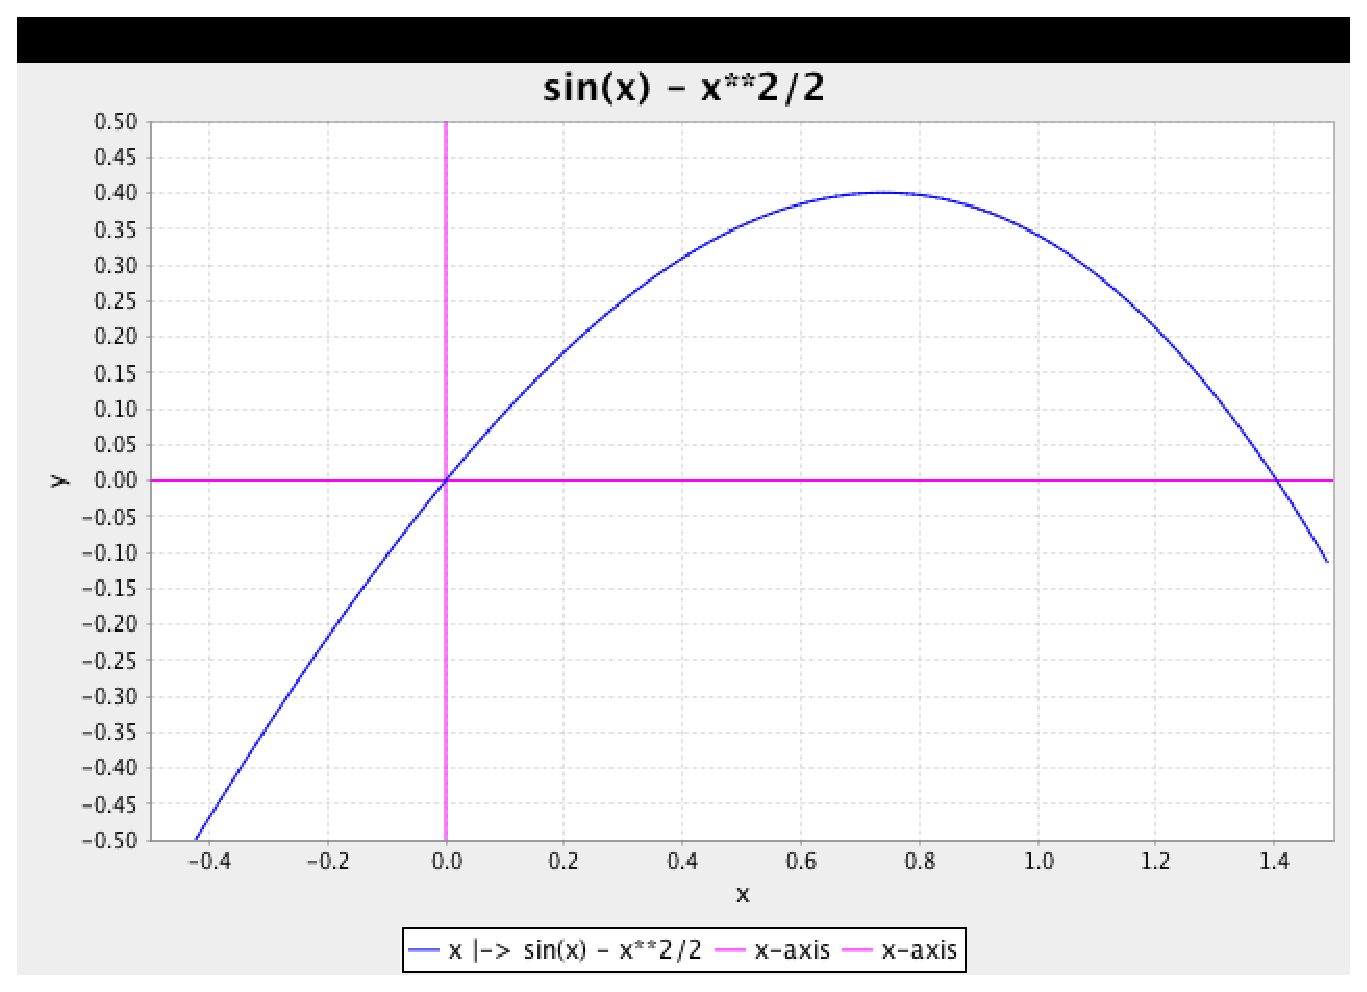
\epsfig{file=Figures/sin-minus-square.eps, scale=0.6}
\vspace*{-0.3cm}
\caption{The function $x \mapsto \sin(x) - \frac{1}{2} \cdot x^2$.}
\label{fig:sin-minus-square.eps}
\end{figure}

\noindent
Unfortunately, in many cases the equation 
\\[0.2cm]
\hspace*{1.3cm}
$\nabla f(\mathbf{\widehat{x}}) = \mathbf{0}$
\\[0.2cm]
can not be solved explicitly.  This is already true in the one-dimensional case, i.e.~if $n=1$.  For example, consider
the function $f:\mathbb{R} \rightarrow \mathbb{R}$ that is defined as
\\[0.2cm]
\hspace*{1.3cm}
$\ds f(x) := \sin(x) - \frac{1}{2} \cdot x^2$.
\\[0.2cm]
This function is shown in Figure \ref{fig:sin-minus-square.eps} on page \pageref{fig:sin-minus-square.eps}.
From the graph of the function it is obvious that this function has a maximum somewhere between $0.6$ and
$0.8$.  In order to compute this maximum, we can compute the derivative of $f$.   This derivative is given as 
\\[0.2cm]
\hspace*{1.3cm}
$f'(x) = \cos(x) - x$
\\[0.2cm]
As it happens, the equation $\cos(x) - x = 0$ does not seem to have a solution in 
\href{https://en.wikipedia.org/wiki/Closed-form_expression}{closed form}.  Hence, we can only approximate
the solution numerically.


The method of \href{https://en.wikipedia.org/wiki/Gradient_descent}{gradient ascent} is a numerical
method that can be used to find the maximum of a function 
\\[0.2cm]
\hspace*{1.3cm}
$f: \mathbb{R}^n \rightarrow \mathbb{R}$.
\\[0.2cm]
The basic idea is to take a vector $\mathbf{x}_0 \in \mathbb{R}^n$ as start value and define a sequence of
vectors $\bigl(\mathbf{x}_n\bigr)_{n\in\mathbb{N}}$ such that we have
\\[0.2cm]
\hspace*{1.3cm}
$f(\mathbf{x}_{n+1}) \geq f(\mathbf{x}_{n})$ \quad for all $n\in\mathbb{N}$.
\\[0.2cm]
Hopefully, this sequence will converge against $\widehat{\mathbf{x}} = \arg\max\limits_{\mathbf{x}\in \mathbb{R}}f(\mathbf{x})$.
If we do not really know where to start our search, we define $\mathbf{x}_0 := \mathbf{0}$.  In order to
compute $\mathbf{x}_{n+1}$ given $\mathbf{x}_{n}$, the idea is to move from $\mathbf{x}_n$ in that direction
where we have the biggest change in the values of $f$.   This direction happens to be the gradient of $f$ at $\mathbf{x}_n$.
Therefore, the definition of $\mathbf{x}_{n+1}$ is given as follows:
\\[0.2cm]
\hspace*{1.3cm}
$\mathbf{x}_{n+1} := \mathbf{x}_n + \alpha \cdot \nabla f(\mathbf{x}_n)$ \quad for all $n \in \mathbb{N}_0$.
\\[0.2cm]
Here, $\alpha$ is called the \blue{step size}.  It determines by how much we move in the direction of the gradient.
In practice, it is best to adapt the step size dynamically during the iteration.  Figure
\ref{fig:gradient-ascent.stlx} shows how this is done.



\begin{figure}[!ht]
\centering
\begin{Verbatim}[ frame         = lines, 
                  framesep      = 0.3cm, 
                  firstnumber   = 1,
                  labelposition = bottomline,
                  numbers       = left,
                  numbersep     = -0.2cm,
                  xleftmargin   = 0.8cm,
                  xrightmargin  = 0.8cm,
                ]
    findMaximum := procedure(f, gradF, start, eps) {
        x     := start;
        fx    := f(x);
        alpha := 1.0;
        while (true) {
            [xOld, fOld] := [x, fx];
            x  += alpha * gradF(x);
            fx := f(x);
            if (fx < fOld) {   
                alpha   *= 0.5;
                [x, fx] := [xOld, fOld];
                continue;  // start over
            } else {
                alpha *= 1.2;
            }
            if (abs(fx - fOld) <= abs(fx) * eps) {
                return [x, fx];
            } 
        }
    };
\end{Verbatim}
\vspace*{-0.3cm}
\caption{The gradient ascent algorithm.}
\label{fig:gradient-ascent.stlx}
\end{figure}

\noindent
The function \texttt{findMaximum} takes four arguments:
\begin{enumerate}
\item \texttt{f} is the function that is to be maximized.  It is assumed that \texttt{f} takes a vector
      $\texttt{x}\in \mathbb{R}^n$ as its input and that it returns a real number.
\item \texttt{gradF} is the gradient of \texttt{f}.  It takes a vector
      $\texttt{x}\in \mathbb{R}^n$ as its input and returns the vector $\nabla \mathtt{f}(\mathtt{x})$.
\item \texttt{start} is the a vector from $\mathbb{R}^n$ that is used as the value of $\mathbf{x}_0$.  In
      practice, we will often use $\mathbf{0} \in \mathbb{R}^n$ as the start vector.
\item \texttt{eps} is the precision that we need for the maximum.  We will have to say more on how \texttt{eps}
      is exactly related to the precision later.  As we are using double precision floating point arithmetic, 
      it won't make sense to use a value for \texttt{eps} that is smaller than $10^{-15}$.
\end{enumerate}
Next, let us discuss the implementation of gradient ascent.
\begin{enumerate}
\item \texttt{x} is initialized with the parameter \texttt{start}.  Hence, \texttt{start} is really the same as
      $\mathbf{x}_0$. 
\item \texttt{fx} is the value that the function $f$ takes for the argument \texttt{x}.
\item \texttt{alpha} is the step size $\alpha$.  We initialize \texttt{alpha} as $1.0$.  It will be adapted
      dynamically. 
\item The \texttt{while} loop starting in line 5 executes the iteration.
\item In each iteration, we store the values of $\mathbf{x}_n$ and $f(\mathbf{x}_n)$ in the variables
      \texttt{xOld} and \texttt{fOld}.
\item Next, we compute $\mathbf{x}_{n+1}$ in line 7 and compute the corresponding value $f(\mathbf{x}_{n+1})$ in line 8.
\item If we are unlucky, $f(\mathbf{x}_{n+1})$ is smaller than $f(\mathbf{x}_{n})$.  This happens if the step
      size $\alpha$ is too large.  Hence, in this case we decrease the value of $\alpha$, discard 
      both $\mathbf{x}_{n+1}$ and $f(\mathbf{x}_{n+1})$ and start over again.
\item Otherwise, $\mathbf{x}_{n+1}$ is a better approximation of the maximum than $\mathbf{x}_n$.  
      In order to increase the speed of the convergence of our algorithm we will then increase the step size
      $\alpha$ by $20\%$.    
\item The idea of our implementation is to stop the iteration when the function values of 
      $f(\mathbf{x}_{n+1})$ and $f(\mathbf{x}_{n})$ do not differ by more than $\varepsilon$ percent, or, to be more
      precise, if
      \\[0.2cm]
      \hspace*{1.3cm}
      $f(\mathbf{x}_{n+1}) < f(\mathbf{x}_{n}) \cdot (1 + \varepsilon)$.
      \\[0.2cm]
      As the sequence $\bigl(f(\mathbf{x}_n\bigr)_{n\in\mathbb{N}}$ will be monotonically
      increasing, i.e.~we have
      \\[0.2cm]
      \hspace*{1.3cm}
      $f(\mathbf{x}_{n+1}) \geq f(\mathbf{x}_{n})$ \quad for all $n\in\mathbb{N}$,
      \\[0.2cm]
      the condition given above is sufficient.  Now, if the increase of  $f(\mathbf{x}_{n+1})$ is less than $f(\mathbf{x}_{n}) \cdot (1 + \varepsilon)$ 
      we assume that we have reached the maximum with the required precision.  In this case we return both the
      value of \texttt{x} and the corresponding function value $f(\mathtt{x})$.
\end{enumerate}
The implementation of gradient ascent given above is not the most sophisticated variant of this algorithm.
It should also be noted that there are algorithms that are more powerful than
gradient ascent.  The first of these methods is the
\href{https://en.wikipedia.org/wiki/Conjugate_gradient_method}{conjugate gradient method}.  A
refinement of this method is the
\href{https://en.wikipedia.org/wiki/Broyden-Fletcher-Goldfarb-Shanno_algorithm}{BFGS-algorithm} that
has been invented by Broyden, Fletcher, Goldfarb, and Shanno.  Unfortunately, we do not have the
time to discuss this algorithm.
However, our implementation of gradient ascent is sufficient for our applications and as this is not a course on numerical
analysis but rather on artificial intelligence we will not delve deeper into this topic but, instead, we refer
readers interested in more efficient algorithms to the literature \cite{snyman:2005}.  If you ever need to find
the maximum of a function numerically, you should try to use a predefined library routine that implements a
state of the art algorithm.


\section{Logistic Regression}
In \href{https://en.wikipedia.org/wiki/Logistic_regression}{logistic regression} we use a linear model that is combined
with the \blue{sigmoid function}.  Before we can discuss the details of logistic regression we need to
define this function and state some of its properties. 

\subsection{The Simoid Function}
\begin{Definition}[Sigmoid Function]
The \href{https://en.wikipedia.org/wiki/Sigmoid_function}{sigmoid function} $S: \mathbb{R} \rightarrow [0, 1]$ is defined as 
\\[0.2cm]
\hspace*{1.3cm}
$\ds S(t) = \frac{1}{1 + \exp(-t)}$.  
\\[0.2cm]
Figure \ref{fig:sigmoid.eps} on page \pageref{fig:sigmoid.eps} shows the sigmoid function.
\eox
\end{Definition}

\begin{figure}[!ht]
\centering
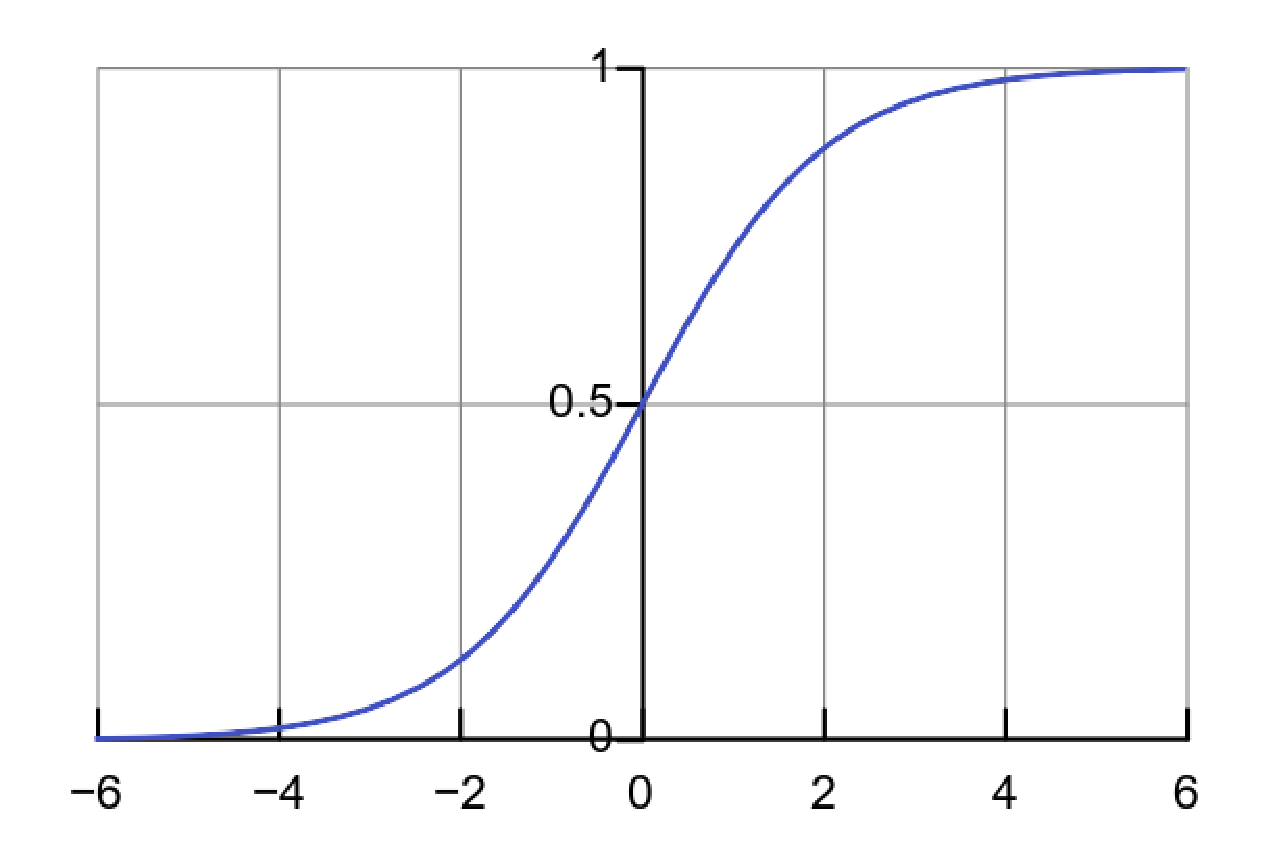
\epsfig{file=Figures/sigmoid.eps, scale=0.7}
\vspace*{-0.3cm}
\caption{The sigmoid function.}
\label{fig:sigmoid.eps}
\end{figure}


\noindent
Let us note some immediate consequences of the definition of the sigmoid function.  As we have
\\[0.2cm]
\hspace*{1.3cm}
$\ds\lim\limits_{x\rightarrow-\infty} \exp(-x) = \infty$, \quad 
$\ds\lim\limits_{x\rightarrow+\infty} \exp(-x) = 0$, \quad and \quad
$\ds\lim\limits_{x\rightarrow\infty} \frac{1}{x} = 0$, 
\\[0.2cm]
the sigmoid function has the following properties:
\\[0.2cm]
\hspace*{1.3cm}
$\ds \lim_{t\rightarrow-\infty} S(t) = 0$ \quad and \quad
$\ds \lim_{t\rightarrow+\infty} S(t) = 1$.
\\[0.2cm]
Another important property is the symmetry of the sigmoid function.  Figure \ref{fig:sigmoid.eps} shows that if the
sigmoid function is shifted down by $\frac{1}{2}$, the resulting function is 
\href{https://en.wikipedia.org/wiki/Point_reflection}{centrally symmetric}, i.e.~we have
\\[0.2cm]
\hspace*{1.3cm}
$\ds S(-t) - \frac{1}{2} = -\Bigl(S(t) - \frac{1}{2}\Bigr)$.
\\[0.2cm]
Adding $\ds\frac{1}{2}$ on both sides of this equation shows that this is equivalent to the equation
\\[0.2cm]
\hspace*{1.3cm}
\colorbox{red}{\framebox{\colorbox{orange}{
$S(-t) = 1 - S(t)$,}}}
\\[0.2cm]
The proof of this fact runs as follows:
\\[0.2cm]
\hspace*{1.3cm}
$
\begin{array}{lcll}
1 - S(t) & = & \ds 1 - \frac{1}{1 + \exp(-t)}             & \mbox{by definition of $S(t)$}           \\[0.5cm]
         & = & \ds \frac{1 + \exp(-t) - 1}{1 + \exp(-t)}  & \mbox{common denominator}                \\[0.5cm]
         & = & \ds \frac{\exp(-t)}{1 + \exp(-t)}          & \mbox{simplify}                          \\[0.5cm]
         & = & \ds \frac{1}{1 + \exp(+t)}                 & \mbox{expand fraction by $\exp(t)$}      \\[0.5cm]
         & = & S(-t). \qquad _\Box                         & \mbox{by definition of $S(-t)$}
\end{array}
$
\\[0.2cm]
The exponential function can be expressed via the sigmoid function.  Let us start with the definition of the sigmoid
function. 
\\[0.2cm]
\hspace*{1.3cm}
$\ds S(t) = \frac{1}{1 + \exp(-t)}$
\\[0.2cm]
Multiplying this equation with the denominator yields
\\[0.2cm]
\hspace*{1.3cm}
$\ds S(t) \cdot \bigl(1 + \exp(-t)\bigr) = 1$.
\\[0.2cm]
Dividing both sides by $S(t)$ gives:
\\[0.2cm]
\hspace*{1.3cm}
$
\begin{array}{cl}
                & \ds 1 + \exp(-t) = \frac{1}{S(t)}        \\[0.5cm]
\Leftrightarrow & \ds \exp(-t) = \frac{1}{S(t)} - 1        \\[0.5cm]
\Leftrightarrow & \ds \exp(-t) = \frac{1 - S(t)}{S(t)}      
\end{array}
$
\\[0.2cm]
We highlight this formula, as we need it later
\\[0.2cm]
\hspace*{1.3cm}
\colorbox{red}{\framebox{\colorbox{orange}{$\ds \exp(-t) = \frac{1 - S(t)}{S(t)}$.}}}
\\[0.2cm]
If we take the reciprocal of both sides of this equation, we have
\\[0.2cm]
\hspace*{1.3cm}
$\ds \exp(t) = \frac{S(t)}{1 - S(t)}$.
\\[0.2cm]
Applying the natural logarithm on both sides of this equation yields
\\[0.2cm]
\hspace*{1.3cm}
$\ds t = \ln\left(\frac{S(t)}{1-S(t)}\right)$.
\\[0.2cm]
This shows that the inverse of the sigmoid function is given as
\\[0.2cm]
\hspace*{1.3cm}
\colorbox{red}{\framebox{\colorbox{orange}{
$\ds S^{-1} (y) = \ln\left(\frac{y}{1-y}\right)$.}}} 
\\[0.2cm]
This function is known as the \href{https://en.wikipedia.org/wiki/Logit}{logit function}.
Next, let us compute the derivative of $S(t)$, i.e.~$\ds S'(t) =\frac{\mathrm{d}S}{\mathtt{d}t}$.  We have
\\[0.2cm]
\hspace*{1.3cm}
$
\begin{array}{lcl}
 S'(t) & = & \ds -\frac{-\exp(-t)}{\bigr(1+\exp(-t)\bigr)^2}   \\[0.5cm]
       & = & \ds \exp(-t) \cdot S(t)^2                       \\[0.2cm]
       & = & \ds \frac{1-S(t)}{S(t)} \cdot S(t)^2            \\[0.4cm]
       & = & \ds \bigl(1 - S(t)\bigr) \cdot S(t)            
\end{array}
$
\\[0.2cm]
We have shown
\\[0.2cm]
\hspace*{1.3cm}
\colorbox{red}{\framebox{\colorbox{orange}{$S'(t) = \bigl(1 - S(t)\bigr) \cdot S(t)$.}}}
\\[0.2cm]
We will later need the derivative of the logarithm of the logistic function.  We define
\\[0.2cm]
\hspace*{1.3cm}
$L(t) := \ln\bigl(S(t)\bigr)$.
\\[0.2cm]
Then we have
\\[0.2cm]
\hspace*{1.3cm}
$
\begin{array}{lcll}
  L'(t) & = & \ds \frac{S'(t)}{S(t)}                  & \mbox{by the chain rule} \\[0.5cm]
        & = & \ds \frac{(1 - S(t)) \cdot S(t)}{S(t)}  \\[0.5cm]
        & = & \ds 1 - S(t)                            \\[0.2cm]
        & = & \ds S(-t)
\end{array}
$
\\[0.2cm]
% If we have the function $f(t) := L(-t)$, then we see that
%\\[0.2cm]
%\hspace*{1.3cm}
% $f'(t) = -S(t)$
%\\[0.2cm]
% holds.   
As this is our most important result, we highlight it:
\\[0.2cm]
\hspace*{1.3cm}
\colorbox{red}{\framebox{\colorbox{orange}{$L'(t) = S(-t)$ \quad where \quad $L(t) := \ln\bigl(S(t)\bigr)$.}}}


\subsection{The Model of Logistic Regression}
We use the following model to compute the probability that an object with features $\mathbf{x}$ will be of the given class:
\\[0.2cm]
\hspace*{1.3cm}
$P(y=+1\;|\;\mathbf{x};\mathbf{w}) = S(\mathbf{x} \cdot \mathbf{w})$.
\\[0.2cm]
Here $\mathbf{x} \cdot \mathbf{w}$ denotes the dot product of the vectors $\mathbf{x}$ and $\mathbf{y}$.  It is
assumed that $\mathbf{x}$ contains a constant feature which  always takes the value of $1$.
Seeing this model the first time you might think that this model is not very general and that it can only be
applied in very special circumstances.  However, the fact is that the features can be functions of arbitrary complexity
and hence this model is much more general than it appears on first sight.

We assume that $y$ can only take the values $+1$ or $-1$,  e.g.~in the example of spam detection $y = 1$ if the
email is spam and $y = -1$ otherwise.  Since complementary probabilities add up to $1$, we have
\\[0.2cm]
\hspace*{1.3cm}
$P(y=-1\;|\;\mathbf{x};\mathbf{w}) = 1 - P(y=+1\;|\;\mathbf{x};\mathbf{w}) 
  = 1 - S(\mathbf{x} \cdot \mathbf{w}) = S(-\mathbf{x} \cdot \mathbf{w})
$.
\\[0.2cm]
Hence, we can combine the equations for $P(y=-1\;|\;\mathbf{x};\mathbf{w})$ and $P(y=+1\;|\;\mathbf{x};\mathbf{w})$ into a
single equation
\\[0.2cm]
\hspace*{1.3cm}
\colorbox{red}{\framebox{\colorbox{orange}{$P(y\;|\;\mathbf{x};\mathbf{w}) = S\bigl(y \cdot(\mathbf{x} \cdot \mathbf{w})\bigr)$.}}}
\\[0.2cm]
Given $N$ objects $o_1, \cdots, o_n $ with feature vectors $\mathbf{x}_1, \cdots, \mathbf{x}_n$ we
want to determine the weight vector $\mathbf{w}$ such that the likelihood $\ell(\mathbf{X}, \mathbf{y})$ of all of our
observations is maximized.  This approach is called the 
\href{https://en.wikipedia.org/wiki/Maximum_likelihood_estimation}{maximum likelihood estimation} of the weights.
As we assume the probabilities of different observations are independent, the individual
probabilities have to be multiplied to compute the overall likelihood $\ell(\mathbf{X}, \mathbf{y};\mathbf{w})$ 
of a given training set:
\\[0.2cm]
\hspace*{1.3cm}
$\ds \ell(\mathbf{X},\mathbf{y};\mathbf{w}) = \prod\limits_{i=1}^N P(y_i \;|\;\mathbf{x}_i;\mathbf{w})$.
\\[0.2cm]
Here, we have combined the different attribute vectors $\mathbf{x}_i$ into the matrix $\mathbf{X}$.  Since it is
easier to work with sums than with products, instead of maximizing the function $\ell(\mathbf{X},\mathbf{y};\mathbf{w})$ we maximize the function
\\[0.2cm]
\hspace*{1.3cm}
$\ell\ell(\mathbf{X},\mathbf{y};\mathbf{w}) := \ln\bigl(\ell(\mathbf{X},\mathbf{y};\mathbf{w})\bigr)$. 
\\[0.2cm]
As the natural logarithm is a monotone function, the functions $\ell(\mathbf{X},\mathbf{y};\mathbf{w})$ and 
$\ell\ell(\mathbf{X},\mathbf{y};\mathbf{w})$ take their maximum at the same value of $\mathbf{w}$.  As we have
\\[0.2cm]
\hspace*{1.3cm}
$\ln(a \cdot b) = \ln(a) + \ln(b)$,
\\[0.2cm]
the natural logarithm of the likelihood is 
\\[0.2cm]
\hspace*{1.3cm}
\colorbox{red}{\framebox{\colorbox{orange}{
$\ds \ell\ell(\mathbf{X},\mathbf{y};\mathbf{w}) = 
 \sum\limits_{i=1}^N \ln\Bigl(S\bigl(y_i \cdot(\mathbf{x}_i \cdot \mathbf{w})\bigr)\Bigr) =
 \sum\limits_{i=1}^N L\bigl(y_i \cdot(\mathbf{x}_i \cdot \mathbf{w})\bigr)
$.}}}
\\[0.2cm]
Our goal is to maximize the likelihood.  Since this is the same as maximizing the log-likelihood, we
need to determine those values of the coefficients $\mathbf{w}$ that satisfy
\\[0.2cm]
\hspace*{1.3cm}
$\ds \frac{\partial\quad}{\partial\, w_j}\ell\ell(\mathbf{X},\mathbf{y};\mathbf{w}) = 0$.
\\[0.2cm]
In order to compute the partial derivative of $\ell\ell(\mathbf{X},\mathbf{y};\mathbf{w})$ with respect to the
coefficients $\mathbf{w}$ we need to compute the partial derivative of the dot product $\mathbf{x}_i \cdot
\mathbf{w}$ with respect to the weights $w_j$.
We define
\\[0.2cm]
\hspace*{1.3cm}
$\ds h(\mathbf{w}) := \mathbf{x}_i \cdot \mathbf{w} = \sum\limits_{k=1}^D x_{i,k} \cdot w_j$.
\\[0.2cm]
Then we have
\\[0.2cm]
\hspace*{1.3cm}
$\ds \frac{\partial\quad}{\partial\, w_j} h(\mathbf{w}) = x_{i,j}$.
\\[0.2cm]
Now we are ready to compute the partial derivative of $\ell\ell(\mathbf{X},\mathbf{y};\mathbf{w})$ with respect to $\mathbf{w}$:
\\[0.2cm]
\hspace*{1.3cm}
$
\begin{array}{cll}
  & \ds \frac{\partial\quad}{\partial\, w_j} \ell\ell(\mathbf{X},\mathbf{y};\mathbf{w}) \\[0.5cm]
= & \ds \frac{\partial\quad}{\partial\, w_j} 
    \sum\limits_{i=1}^N L\bigl(y_i \cdot(\mathbf{x}_i \cdot \mathbf{w})\bigr) 
    \\[0.5cm]
= & \ds\sum\limits_{i=1}^N y_i \cdot x_{i,j} \cdot  S\bigl(-y_i \cdot(\mathbf{x}_i \cdot \mathbf{w})\bigr),
  & \mbox{since} \quad \ds \frac{\mathrm{d}L(x)}{\mathrm{d}x} = S(-x).
\end{array}
$
\\[0.2cm]
Hence, the partial derivative of the log-likelihood function is given as follows:
\\[0.2cm]
\hspace*{1.3cm}
\colorbox{red}{\framebox{\colorbox{orange}{
$\ds \frac{\partial\quad}{\partial\, w_j}\ell\ell(\mathbf{X},\mathbf{y};\mathbf{w}) =
 \ds\sum\limits_{i=1}^N y_i \cdot x_{i,j} \cdot  S(-y_i \cdot \mathbf{x}_i \cdot \mathbf{w})
$}}} 
\\[0.2cm]
Next, we have to find the value of $\mathbf{w}$ such that
\\[0.2cm]
\hspace*{1.3cm}
$\ds\sum\limits_{i=1}^N y_i \cdot x_{i,j} \cdot  S(-y_i \cdot \mathbf{x}_i \cdot \mathbf{w}) = 0$
\quad for all $j \in \{1, \cdots, D\}$.
\\[0.2cm]
These are $D$ equation for the $D$ variables $w_1, \cdots w_D$.  Due to the occurrence of the sigmoid function, these
equations are nonlinear.  We can not solve these equations explicitly.  Nevertheless, our computation of the
gradient of the log-likelihood was not for nought:  We will use gradient ascent in order to find the value of
$\mathbf{w}$ that maximizes the log-likelihood.
This method has been outlined in the previous section.

\subsection{Implementing Logistic Regression}
In order to implement logistic regression we need a data structure for tabular data.  Figure
\ref{fig:table.stlx} on page \pageref{fig:table.stlx} shows the class table that can be used to
administer this kind of data.  Figure \ref{fig:table.stlx}  shows an example of tabular data that is
stored in a \href{https://en.wikipedia.org/wiki/Comma-separated_values}{csv file}.  In this case,
the data stores the hours a student has learned for a particular exam and the fact whether the
student has passed of failed.  The first column stores pass or fail, where a pass is coded using the
number 1, while a fail is coded as 0.  The second column stores the number of hours that the student
has learned in order to pass the exam.

\begin{figure}[!ht]
\centering
\begin{Verbatim}[ frame         = lines, 
                  framesep      = 0.3cm, 
                  firstnumber   = 1,
                  labelposition = bottomline,
                  numbers       = left,
                  numbersep     = -0.2cm,
                  xleftmargin   = 0.8cm,
                  xrightmargin  = 0.8cm,
                ]
   class table(columnNames, types, data) {
       mColumnNames := columnNames;
       mTypes       := types;
       mData        := data;
   
     static {
         getColumnNames := [ ] |-> mColumnNames;
         getTypes       := [ ] |-> mTypes;
         getData        := [ ] |-> mData;
         getRow         := [r] |-> mData[r];
         getLength      := []  |-> #mData;
         
         head := procedure(limit := 10) {
             print(mColumnNames);
             print(mTypes);
             for (i in [1 .. limit]) {
                 print(mData[i]);
             }
         };
     }
   }
   readTable := procedure(fileName, types) {
       all := readFile(fileName);
       columnNames := split(all[1], ',\s*');
       data := [];
       for (i in [2 .. #all]) {
           row := split(all[i], ',\s*');
           data[i-1] := [eval("$type$($s$)") : [type, s] in types >< row];
       }
       return table(columnNames, types, data);
   };
\end{Verbatim}
\vspace*{-0.3cm}
\caption{A class to represent tabular data.}
\label{fig:table.stlx}
\end{figure}
There is no need for us to discuss every detail of the implementation of the class \texttt{table}.
The important thing to note is that the data is stored as a list of lists in the member variable
\texttt{mData}.  Each of the inner lists corresponds to one row of the csv file.
This member variable can be accessed using the function getData.  The function \texttt{readTable}
has the responsibility to read a csv file and to convert it into an object of class \texttt{table}.
In order to do this, it has to be called with two arguments.  The first argument is the file name,
the second argument is a list of the types of each column in the csv file.  For example, to read the
file ``\texttt{exam.csv}'' we would call \texttt{readTable} as follows:
\\[0.2cm]
\hspace*{1.3cm}
\texttt{readTable("exam.csv", ["int", "double"])}.



\begin{figure}[!ht]
\centering
\begin{Verbatim}[ frame         = lines, 
                  framesep      = 0.3cm, 
                  firstnumber   = 1,
                  labelposition = bottomline,
                  numbers       = left,
                  numbersep     = -0.2cm,
                  xleftmargin   = 0.8cm,
                  xrightmargin  = 0.8cm,
                ]
   Pass, Hours
   0,    0.50
   0,    0.75
   0,    1.00
   0,    1.25
   0,    1.50
   0,    1.75
   1,    1.75
   0,    2.00
   1,    2.25
   0,    2.50
   1,    2.75
   0,    3.00
   1,    3.25
   0,    3.50
   1,    4.00
   1,    4.25
   1,    4.50
   1,    4.75
   1,    5.00
   1,    5.50
\end{Verbatim}
\vspace*{-0.3cm}
\caption{Results of an exam.}
\label{fig:exam.csv}
\end{figure}

The program shown in Figure \ref{fig:logistic-regression.stlx} on page
\pageref{fig:logistic-regression.stlx} implements logistic regression.  As there are a number of
subtle points that might easily be overlooked otherwise, we proceed to discuss this program line by line. 


\begin{figure}[!ht]
\centering
\begin{Verbatim}[ frame         = lines, 
                  framesep      = 0.3cm, 
                  firstnumber   = 1,
                  labelposition = bottomline,
                  numbers       = left,
                  numbersep     = -0.2cm,
                  xleftmargin   = 0.8cm,
                  xrightmargin  = 0.8cm,
                ]
   load("table.stlx");
   load("gradient-ascent.stlx");
   
   sigmoid := procedure(x) { return 1.0 / (1.0 + exp(-x)); };
   logSigmoid := procedure(x) {
       if (x >= -100) {
           return -log(1.0 + exp(-x));
       } else {  
           return x;
       }
   };
   ll := procedure(X, y, w) {
       result := 0;
       for (i in [1 .. #X]) {
           result += logSigmoid(y[i] * (X[i] * w));
       }
       return result;
   };   
   gradLL := procedure(X, y, w) {
       result := [];
       for (j in [1 .. #X[1]]) {
           result[j] := 0;
           for (i in [1 .. #X]) {
               result[j] += y[i] * X[i][j] * sigmoid((-y[i]) * (X[i] * w));
           }
       }
       return la_vector(result);
   };
   logisticRegressionFile := procedure(fileName, types) {
       csv    := readTable(fileName, types);
       data   := csv.getData();
       number := #data;
       dmnsn  := #data[1];    
       yList  := [];
       xList  := [];
       for (i in [1 .. number]) {
           yList[i] := data[i][1];
           xList[i] := la_vector([1.0] + data[i][2..]);
       }
       X := la_matrix(xList);
       y := la_vector([2 * y - 1 : y in yList]);
       start := la_vector([0.0 : i in [1 .. dmnsn]]);
       eps   := 10 ** -15;
       f     := w |=> ll(X, y, w);
       gradF := w |=> gradLL(X, y, w);
       return findMaximum(f, gradF, start, eps)[1];
   };
\end{Verbatim}
\vspace*{-0.3cm}
\caption{An implementation of logistic regression.}
\label{fig:logistic-regression.stlx}
\end{figure}

\begin{enumerate}
\item First, we have to load both the class \texttt{table} and our implementation of gradient ascent 
      that has already been discussed in Section \ref{section:gradient-ascent}.
\item Line 4 implements the sigmoid function
      \\[0.2cm]
      \hspace*{1.3cm}
      $\ds S(x) = \frac{1}{1 + \exp(-x)}$.
\item Line 5 starts the implementation of the natural logarithm of the sigmoid function, i.e.~we implement
      \\[0.2cm]
      \hspace*{1.3cm}
      $\ds L(x) = \ln\bigl(S(X)\bigr) = \ln\left(\frac{1}{1 + \exp(-x)}\right) =- \ln\bigl(1 + \exp(-x)\bigr)$.
      \\[0.2cm]
      The implementation is more complicated than you might expect.  The reason has to do with
      overflow.  Consider values of $x$ that are smaller than, say, $-1000$.  The problem is that
      the expression $\mathtt{exp}(1000))$ evaluates to \texttt{Infinity}, which represents the
      mathematical value $\infty$.  But then $1 + \mathtt{exp}(1000))$ is also \texttt{Infinity} and
      finally \texttt{log(1 + exp(1000))} is \texttt{Infinity}.  However, in reality we have
      \\[0.2cm]
      \hspace*{1.3cm}
      $\ln\bigl(1 + \exp(1000)\bigr) \approx 1000$.
      \\[0.2cm] 
      The argument works as follows:
      \pagebreak
      \vspace*{\fill}

      \pagebreak

      \noindent
      \hspace*{1.3cm}
      $
      \begin{array}{lcll}
        \ln\bigl(1+\exp(x)\bigr) & = & \ln\bigl(\exp(x) \cdot (1+\exp(-x))\bigr)          \\[0.2cm]
                                 & = & \ln\bigl(\exp(x)\bigr) + \ln\bigl(1+\exp(-x)\bigr) \\[0.2cm]
                                 & = & x + \ln\bigl(1+\exp(-x)\bigr) \\[0.2cm]
                                 & \approx & x + \ln(1) + \exp(-x) & \mbox{Taylor expansion of $\ln(1+x)$} \\[0.2cm]
                                 & = & x + 0 + \exp(-x)                                      \\[0.2cm]
                                 & \approx & x                & \mbox{since $\exp(-x) \approx 0$ for large $x$} 
      \end{array}
      $
      \\[0.2cm]
      This is the reason that \texttt{logSigmoid} returns \texttt{x} if \texttt{x} is less than
      $-100$.
\item The function $\mathtt{ll}(\mathbf{x}, \mathbf{y}, \mathbf{w})$ computes the log-lokelihood
      $\ds \ell\ell(\mathbf{X},\mathbf{y};\mathbf{w}) = 
           \sum\limits_{i=1}^N L\bigl(y_i \cdot(\mathbf{x}_i \cdot \mathbf{w})\bigr)
      $.
      Here $L$ denotes the natural logarithm of the sigmoid of the argument.
      It is assumed that $\mathbf{X}$ is a matrix.  Every observation corresponds to a row in this
      matrix, i.e.~the vector $\mathbf{x}_i$ is the feature vector containing the features of the
      $i$-th observation.  $\mathbf{y}$ is a vector describing the outcomes, i.e.~the elements
      of this vector are either $+1$ or $-1$.  Finally, $\mathbf{w}$ is the vector of coefficients.
\item The function $\mathtt{gradLL}(\mathbf{x}, \mathbf{y}, \mathbf{w})$ computes the gradient of
      the log-lokelihood according to the formula
      \\[0.2cm]
      \hspace*{1.3cm}
      $\ds \frac{\partial\quad}{\partial\, w_j}\ell\ell(\mathbf{X},\mathbf{y};\mathbf{w}) =
        \ds\sum\limits_{i=1}^N y_i \cdot x_{i,j} \cdot  S(-y_i \cdot \mathbf{x}_i \cdot \mathbf{w})
      $.
      \\[0.2cm]
      The different components of this gradient are combined into a vector.
      The arguments are the same as the arguments to the log-lokelihood.
\item Finally, the function \texttt{logisticRegressionFile} takes two arguments.  The first argument
      is the name of the csv file containing the data, while the second argument is a list specifying the types
      of the columns.  The elements of this list have to be either \texttt{"int"} or
      \texttt{"double"}.
      The task of this function is to read the csv file, convert the data in the matrix $\mathbf{X}$
      and the vector $\mathtt{y}$, and then use the method of gradient ascent to find the coefficients
      $\mathtt{w}$ that maximize the likelihood.
\end{enumerate}
If we run the function \texttt{logisticRegressionFile} using the data shown in Figure
\ref{fig:exam.csv} via
the command
\\[0.2cm]
\hspace*{1.3cm}
\texttt{logisticRegressionFile("exam.csv", ["int", "double"]);}
\\[0.2cm]
the resulting coefficients are:
\\[0.2cm]
\hspace*{1.3cm}
\texttt{<<-4.077649741107752 1.5046211108850898>>}
\\[0.2cm]
This shows that the probability $P(h)$ that a student who has studied for $h$ hours will pass the
exam is given approximately as follows:
\\[0.2cm]
\hspace*{1.3cm}
$\ds P(h) \approx \frac{1}{1 + \exp(4.1 - 1.5 \cdot h)}$
\\[0.2cm]
Figure \ref{fig:exam-pass.eps} shows a plot of the probability $P(x)$.  This
figure has been taken from the
\href{https://en.wikipedia.org/wiki/Logistic_regression#Fields_and_example_applications}{Wikipedia article on logistic regression}. 
It has been created by \href{https://commons.wikimedia.org/w/index.php?curid=42442194}{Michaelg2015}.


\begin{figure}[!th]
\centering
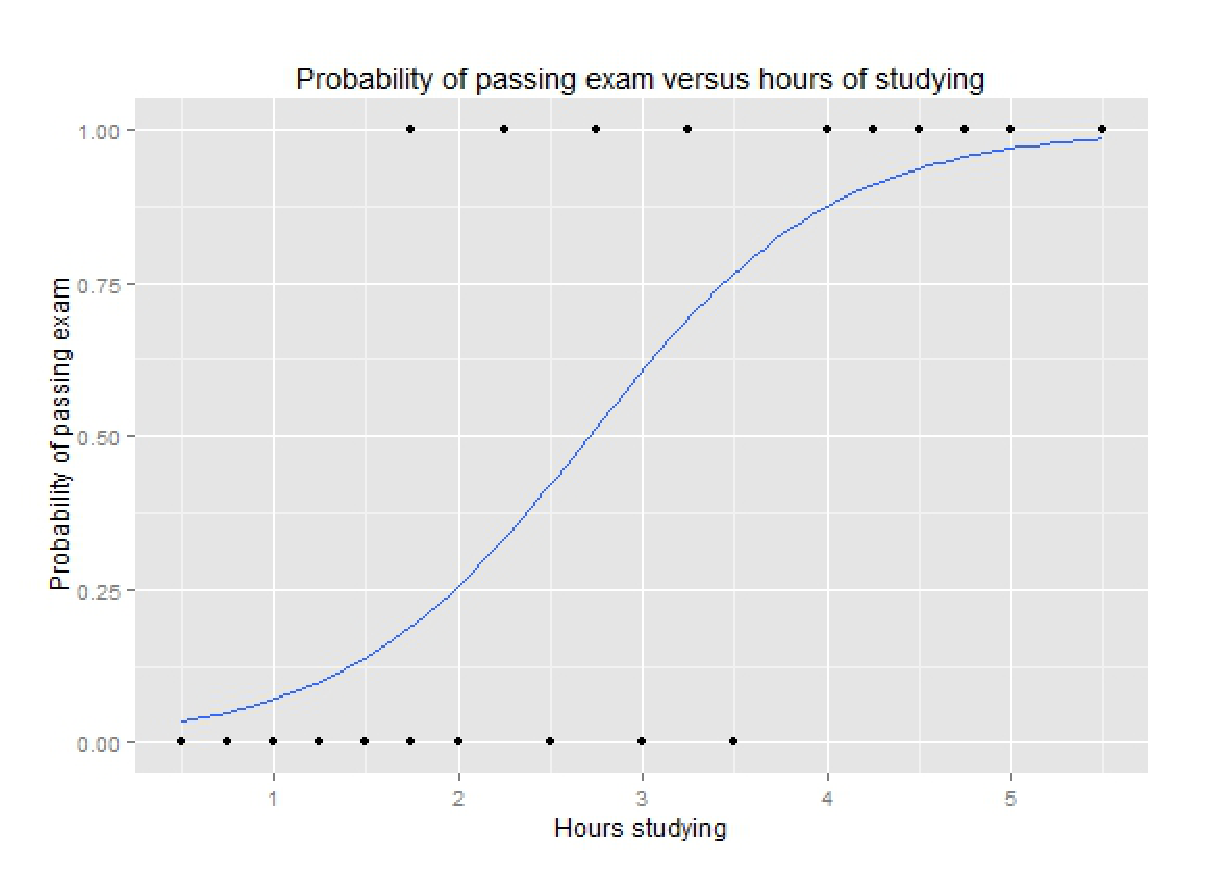
\epsfig{file=Figures/exam-pass.eps, scale=0.6}
\vspace*{-0.3cm}
\caption{Probability of passing an exam versus hours of studying.}
\label{fig:exam-pass.eps}
\end{figure}


%\section{Decision Tree Learning}

%%% Local Variables:
%%% mode: latex
%%% TeX-master: "artificial-intelligence"
%%% End:
